\section{Durchführung}
\label{sec:Durchführung}

Im ersten Teil des Versuchs werden Auf- und Entladevorgang des Kondensators
im RC-Kreis untersucht. Dazu wird ein Versuchsaufbau gemäß Abbildung \ref{fig:aufbau1}
verwendet. 

\begin{figure}
\centering
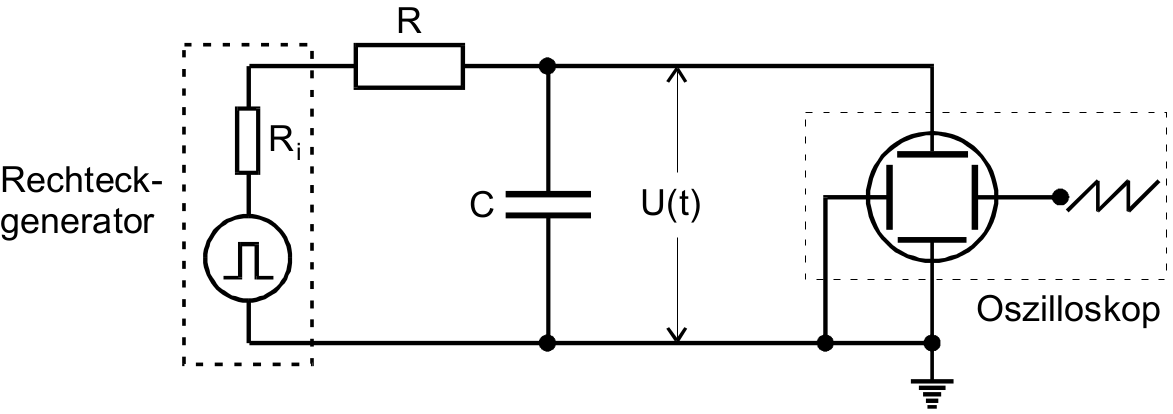
\includegraphics[scale=0.2]{content/aufbau1.png}
\caption{Schaltung zur Beobachtung des Auf- und Entladevorganges des Kondensators [1]}
\label{fig:aufbau1}
\end{figure}

Durch die angelegte Rechteckspannung entlädt und lädt sich der Kondensator 
abwechselnd. Dadurch sind auf dem Oszilloskop beide Vorgänge zu sehen. Es 
werden 10 Messwertpaare von $U_C$ und $t$ eines Ent- oder Aufladevorganges
aufgenommen.  

Im zweitem Teil des Versuchs wird die Frequenzabhängigkeit der Ampflitude der 
Kondensatorspannung untersucht. Dazu wird eine Schaltung gemäß Abbildung \ref{fig:aufbau2}
verwendet. 

\begin{figure}
\centering
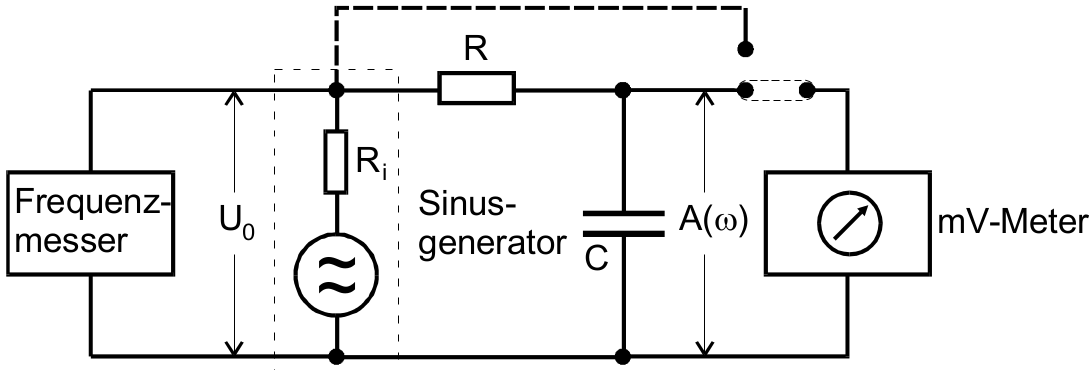
\includegraphics[scale=0.2]{content/aufbau2.png}
\caption{Schaltung zur Untersuchung der Frequenzabhängigkeit der Kondensatorspannungsamplitude [1]}
\label{fig:aufbau2}
\end{figure}

Mit einem Millivoltmeter wird die Kondensatorspannungsamplitude in Abhängigkeit von 
der Frequenz im Bereich über drei Größenordnungen gemessen. Bei der Wahl des 
Frequenzbereiches ist darauf zu achten, dass $U_0$ in diesem von der Frequenz 
nahezu abhängig sein soll. 

Im dritten Versuchsteil wird die Phasenverschiebung zwischen Generator - und 
Kondensatorspannung gemessen. Dazu wird eine Schaltung gemäß Abbildung \ref{fig:aufbau3}
verwendet. 

\begin{figure}
\centering
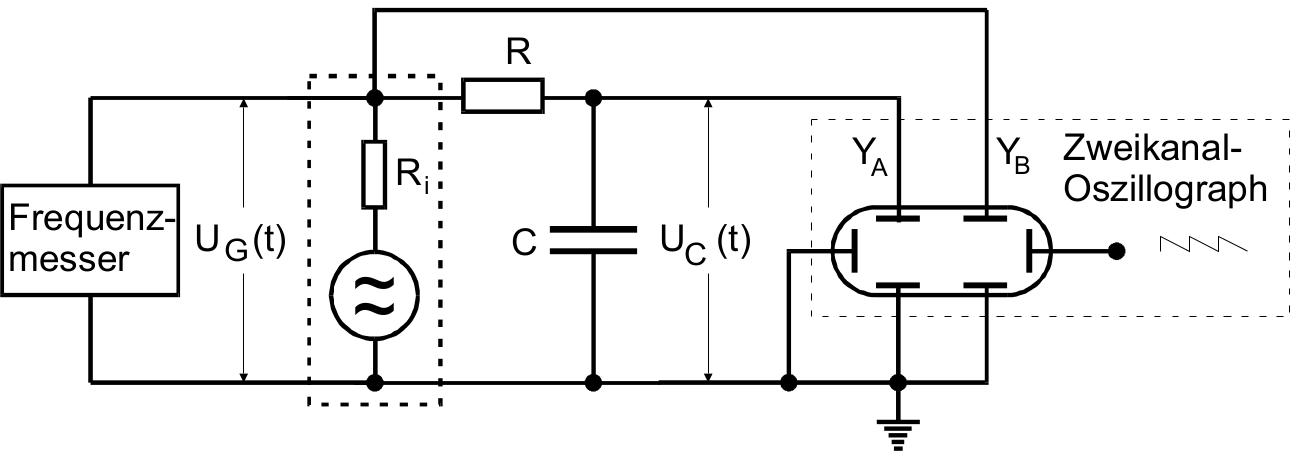
\includegraphics[scale=0.2]{content/aufbau3.png}
\caption{Schaltung zur Untersuchung der Phasenverschiebung zwischen $U(t)$ und $U_C(t)$ [1]}
\label{fig:aufbau3}
\end{figure}

Dafür wird nun die Kondensatorspannung $U_C$ auf den einen Eingang des 
Zweikanaloszilloskops gegeben und die Generatorspannung $U$ auf den anderen. 
Nun wird der zeitliche Abstand der Maxima der beiden Schwingungen gemessen. 

Im letztem Versuchsteil soll gezeigt werden, dass ein RC-Kreis als Integrator 
genutzt werden kann. Dazu wird bei einer Frequenz mit $\omega \gg \frac{1}{RC}$ 
jeweils eine Rechtecks-, Sinus- und Dreiecksspannung auf das RC-Glied gegeben. 
Es werden sowohl Eingangs - als auch Ausgangsspannung auf dem Bildschirm des 
Zweikanaloszilloskops dargestellt und für jede der drei Spannungen ein Bild der 
Signale aufgenommen. 


